\documentclass[11pt,letterpaper]{article}
\usepackage[margin=0.5in]{geometry}
\usepackage{amsmath}
\usepackage{graphicx}
\usepackage{booktabs}
\usepackage{siunitx}
\usepackage{xcolor}
\usepackage{caption}
\usepackage{array}
\usepackage{hyperref}
\usepackage{lastpage}
\usepackage{fancyhdr}
\usepackage[utf8]{inputenc}

\hypersetup{colorlinks=true, linkcolor=blue!50!black, urlcolor=blue!50!black}
\pagestyle{fancy}\fancyhf{}
\rhead{\small Validation Report}
\lhead{\small Halle CTX-500 Transcranial Bowl @ 500 kHz}
\cfoot{\small Page \thepage\ of \pageref{LastPage}}

\setlength{\parskip}{4pt}
\setlength{\parindent}{0pt}

\title{Output Validation Report\\\large Halle CTX-500 Transcranial Bowl @ 500 kHz}
\author{\texttt{halle\_bowl}}
\date{2026-05-01T18:07:01-04:00}

\newcommand{\figref}[1]{\textbf{Figure~\ref{#1}}}

\graphicspath{{figures/}}
\begin{document}
\maketitle
\thispagestyle{fancy}

\section*{Scope}
This report validates the inputs and outputs of a single Fullwave acoustic +
shear-wave simulation. Section~\ref{sec:acoustic_inputs} covers the inputs to
the acoustic FDTD; subsequent sections (added incrementally) will cover
acoustic outputs, acoustic-radiation force, shear inputs, and displacement
outputs.

\section{Acoustic Inputs}\label{sec:acoustic_inputs}

\subsection{Parameters at a glance}\label{sec:params_compact}

\begin{table}[h!]
\centering
\scriptsize
\setlength{\tabcolsep}{4pt}
\renewcommand{\arraystretch}{1.05}
\begin{minipage}[t]{0.32\linewidth}\centering
\textbf{Grid \& timing}\\[2pt]
\begin{tabular}{lr}
\toprule
$f_0$               & 500 kHz \\
$c_0$               & 1540 m/s \\
PPW                 & 10 \\
CFL                 & 0.20 \\
$dx$                & 0.308 mm \\
$dt$                & 40.00 ns \\
Domain              & 65 $\times$ 66 $\times$ 66 mm \\
Voxels              & 211$\times$214$\times$214 \\
$n_T$               & 2110 \\
Sim time            & 84.4 $\mu$s \\
\bottomrule
\end{tabular}
\end{minipage}\hfill
\begin{minipage}[t]{0.32\linewidth}\centering
\textbf{Source spec}\\[2pt]
\begin{tabular}{lr}
\toprule
Type             & tips\_bowl \\
$R_{\text{outer}}$ & 32.0 mm \\
$R_{\text{inner}}$ & 0.0 mm \\
ROC ($F$)        & 63.0 mm \\
Elements         & 4 \\
Layers           & 3 \\
$p_0$            & 0.40 MPa \\
Cycles           & 2 \\
Drop-off         & 2.0 \\
Voxels           & 73638 \\
\bottomrule
\end{tabular}
\end{minipage}\hfill
\begin{minipage}[t]{0.32\linewidth}\centering
\textbf{Placement}\\[2pt]
\begin{tabular}{lr}
\toprule
Scalp            & F3 \\
Target           & DLPFC\_left \\
Req. $F$         & 63 mm \\
Req. $R$         & 32 mm \\
Perp residual    & 1.10 mm \\
Scalp$\to$tgt    & 14.2 mm \\
Apex$\to$tgt     & 22.9 mm \\
Sagitta          & 8.7 mm \\
EEG offset       & 16.4 mm \\
$\hat n_{3D}$    & (-0.68, -0.37, -0.63) \\
\bottomrule
\end{tabular}
\end{minipage}
\caption{FDTD grid (left), bowl source spec (center), and anatomical placement (right). Placement is derived via the SyN MNI$\to$Halle warp from the requested 10-20 scalp site to the requested cortical target.}
\end{table}


\begin{figure}[h!]\centering
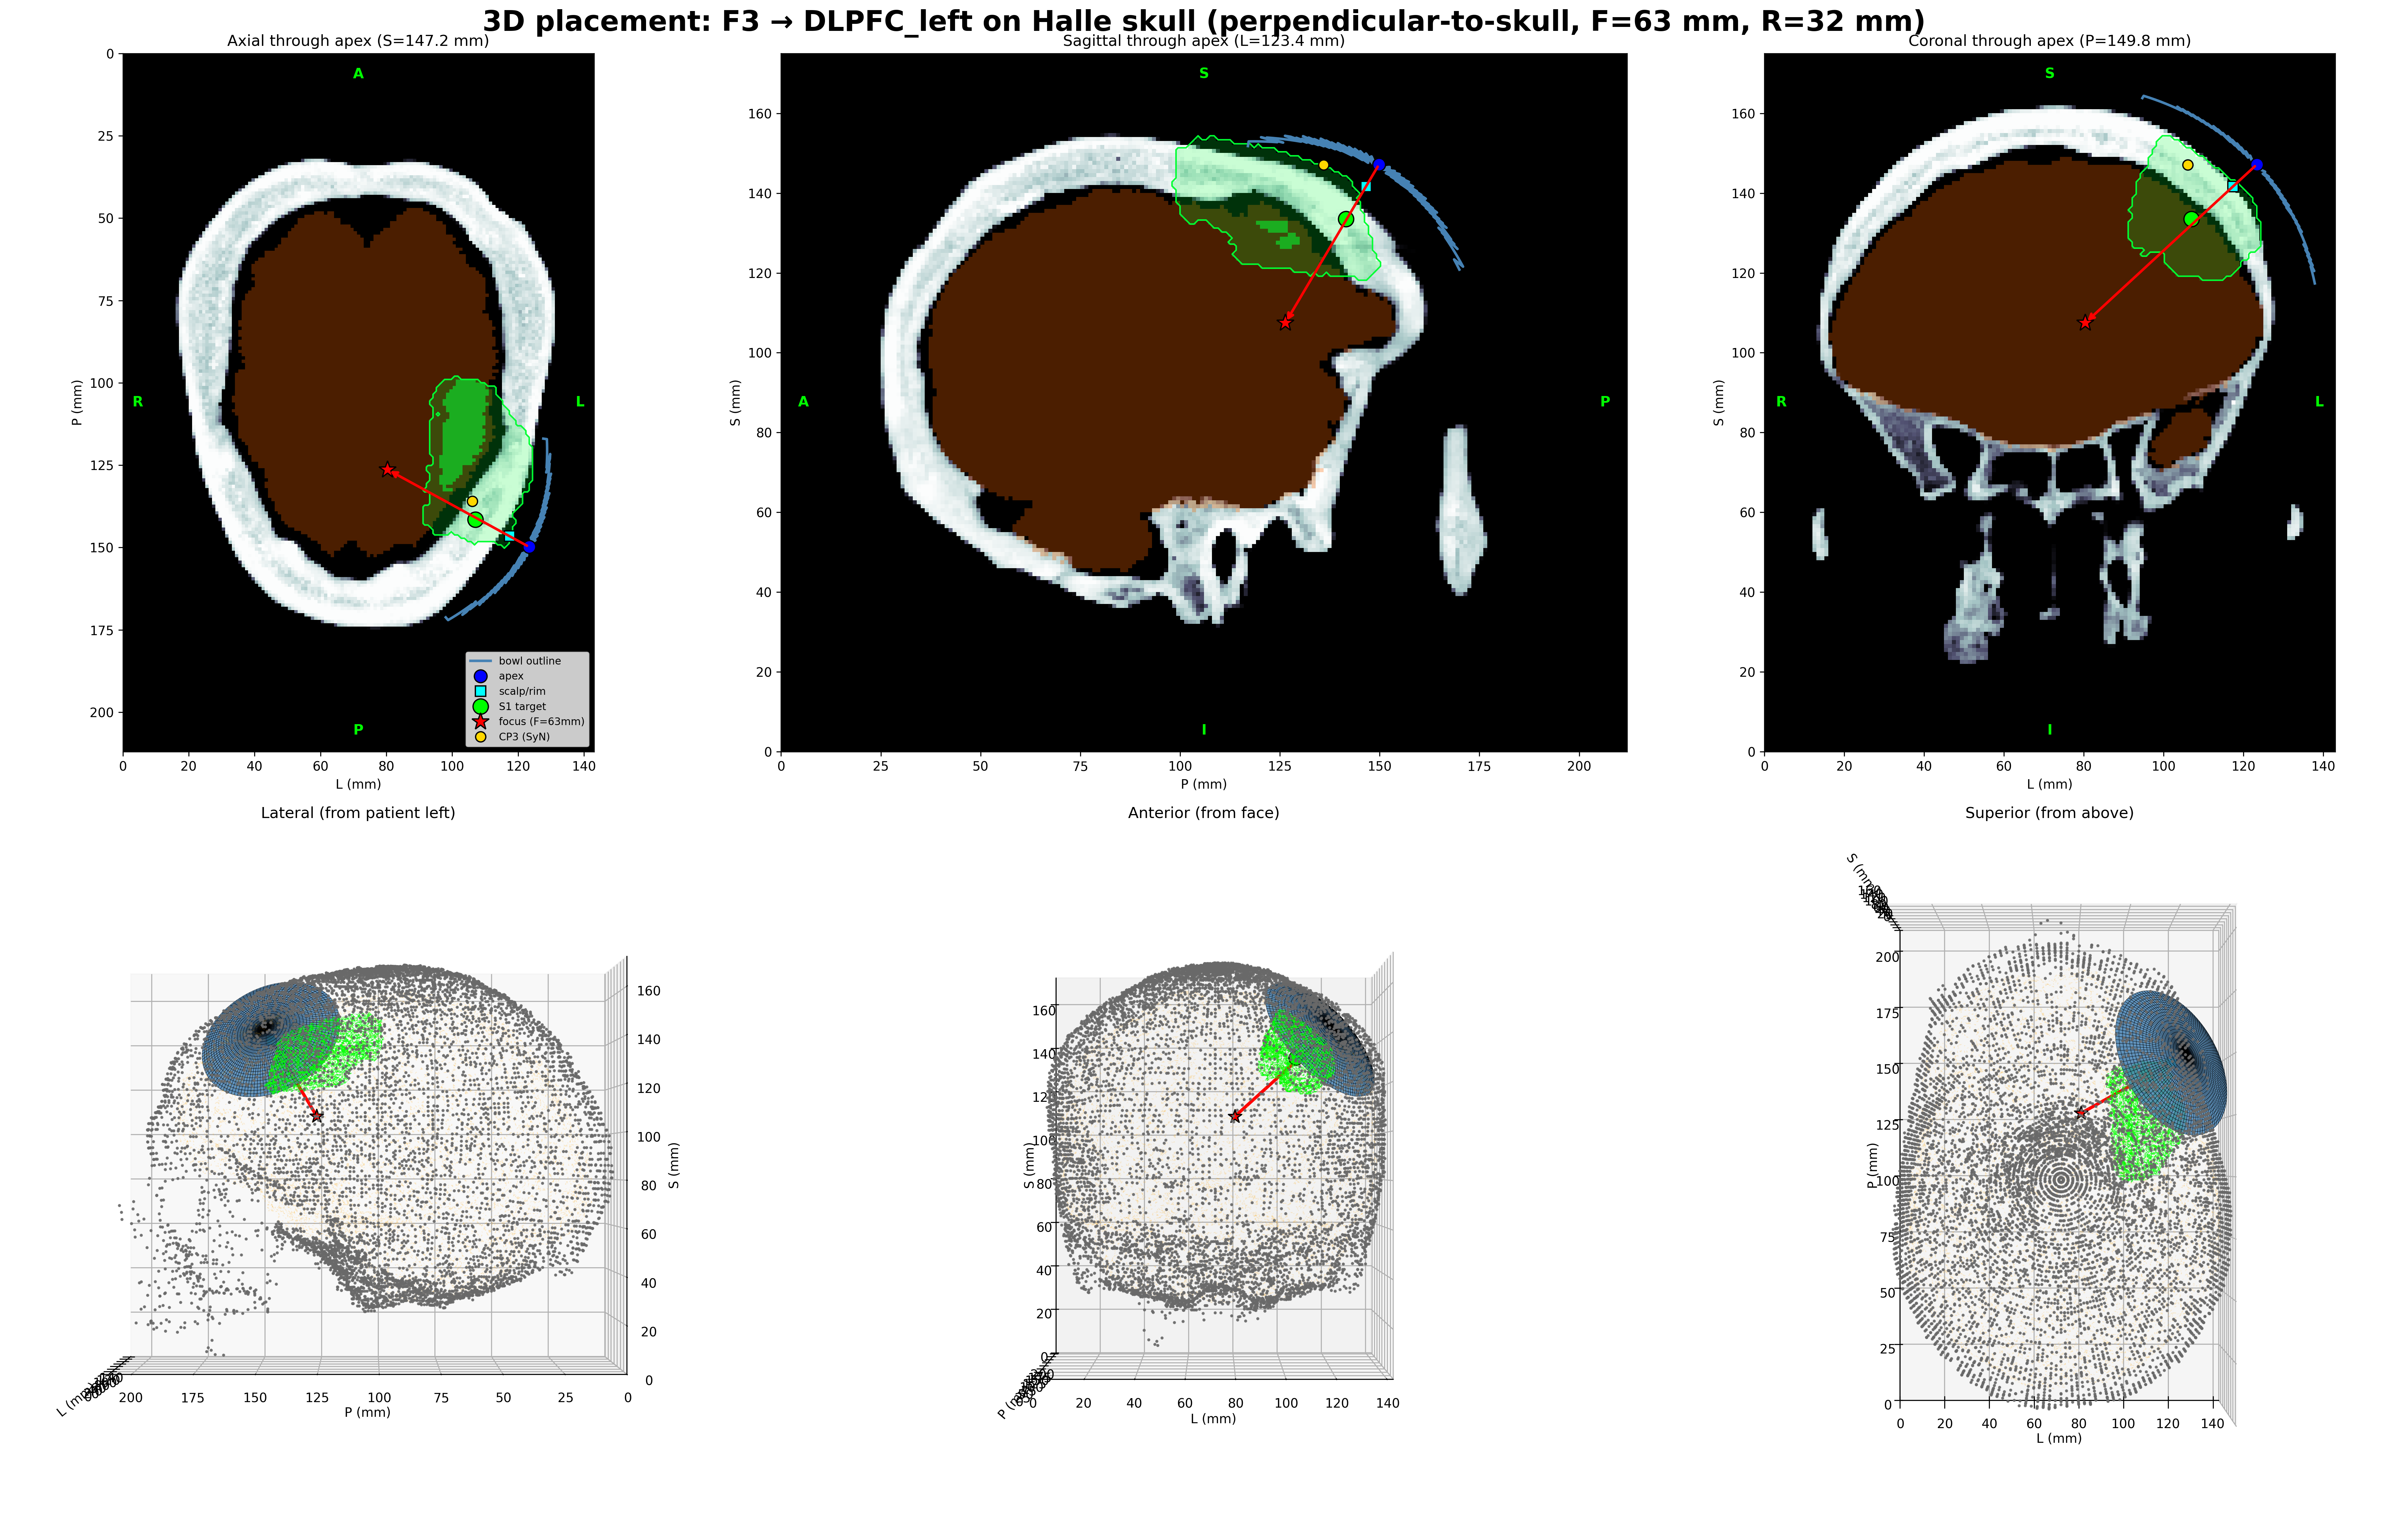
\includegraphics[width=0.95\linewidth]{fig_inputs_placement_3d.png}
\caption{\large\textbf{F3 $\to$ DLPFC\_left: 3D placement on the Halle skull.}\\
\normalsize Top row: orthogonal slice views with bowl outline drawn in plane. Bottom row: three 3D camera angles with bowl wireframe, outer-bone surface, pial brain mesh, and target ROI (Harvard-Oxford label warped to subject space).}\label{fig:placement_3d}
\end{figure}


\begin{figure}[h!]\centering
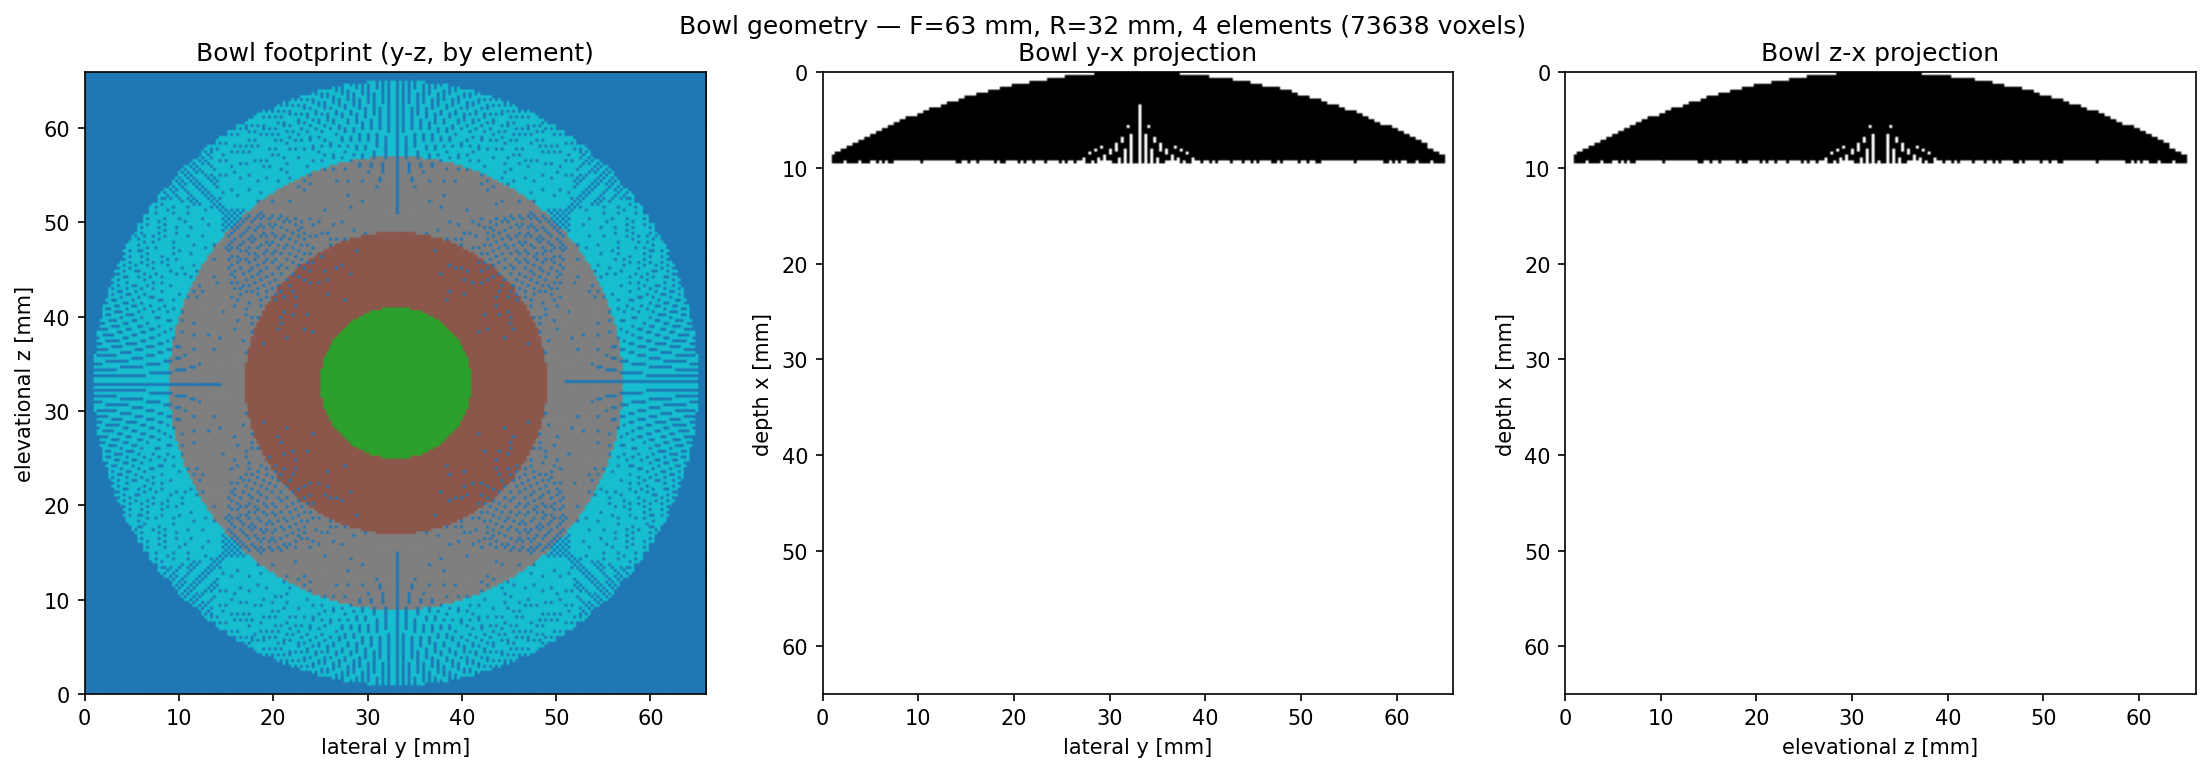
\includegraphics[width=\linewidth]{fig_inputs_bowl_geometry.png}
\caption{Bowl source mask on the FDTD slab grid: y-z aperture footprint colored by annular element (left), x-y projection (middle), x-z projection (right).}\label{fig:bowl_geom}
\end{figure}

\subsection{Acoustic medium}\label{sec:medium}
\begin{table}[h!]
\centering
\scriptsize
\setlength{\tabcolsep}{6pt}
\begin{tabular}{lr|lr}
\toprule
NRRD source        & \texttt{\textasciitilde{}/.cache/fullwave25/skull\_microCT\_zenodo/halle\_skull.nrrd} & HU thresholds        & 700 -- 1973 \\
Speed range req.   & 1540 -- 2900 m/s & Density range req.   & 1000 -- 2200 kg/m\(^3\) \\
Blur $\sigma$      & 0.00 mm & Background           & tissue \\
Built $c$ extent   & 1540 -- 2900 m/s & Built $\rho$ extent  & 1000 -- 2200 kg/m\(^3\) \\
Built $\alpha$ ext.& 0.50 -- 20.00 dB/(MHz cm) & Skull voxels         & 756180 \\
Built $\beta$ ext. & 4.80 -- 5.50 (dimensionless) & & \\
\bottomrule
\end{tabular}
\caption{Medium-builder configuration and resulting voxel-property extents on the slab grid.}
\end{table}

\begin{figure}[h!]\centering
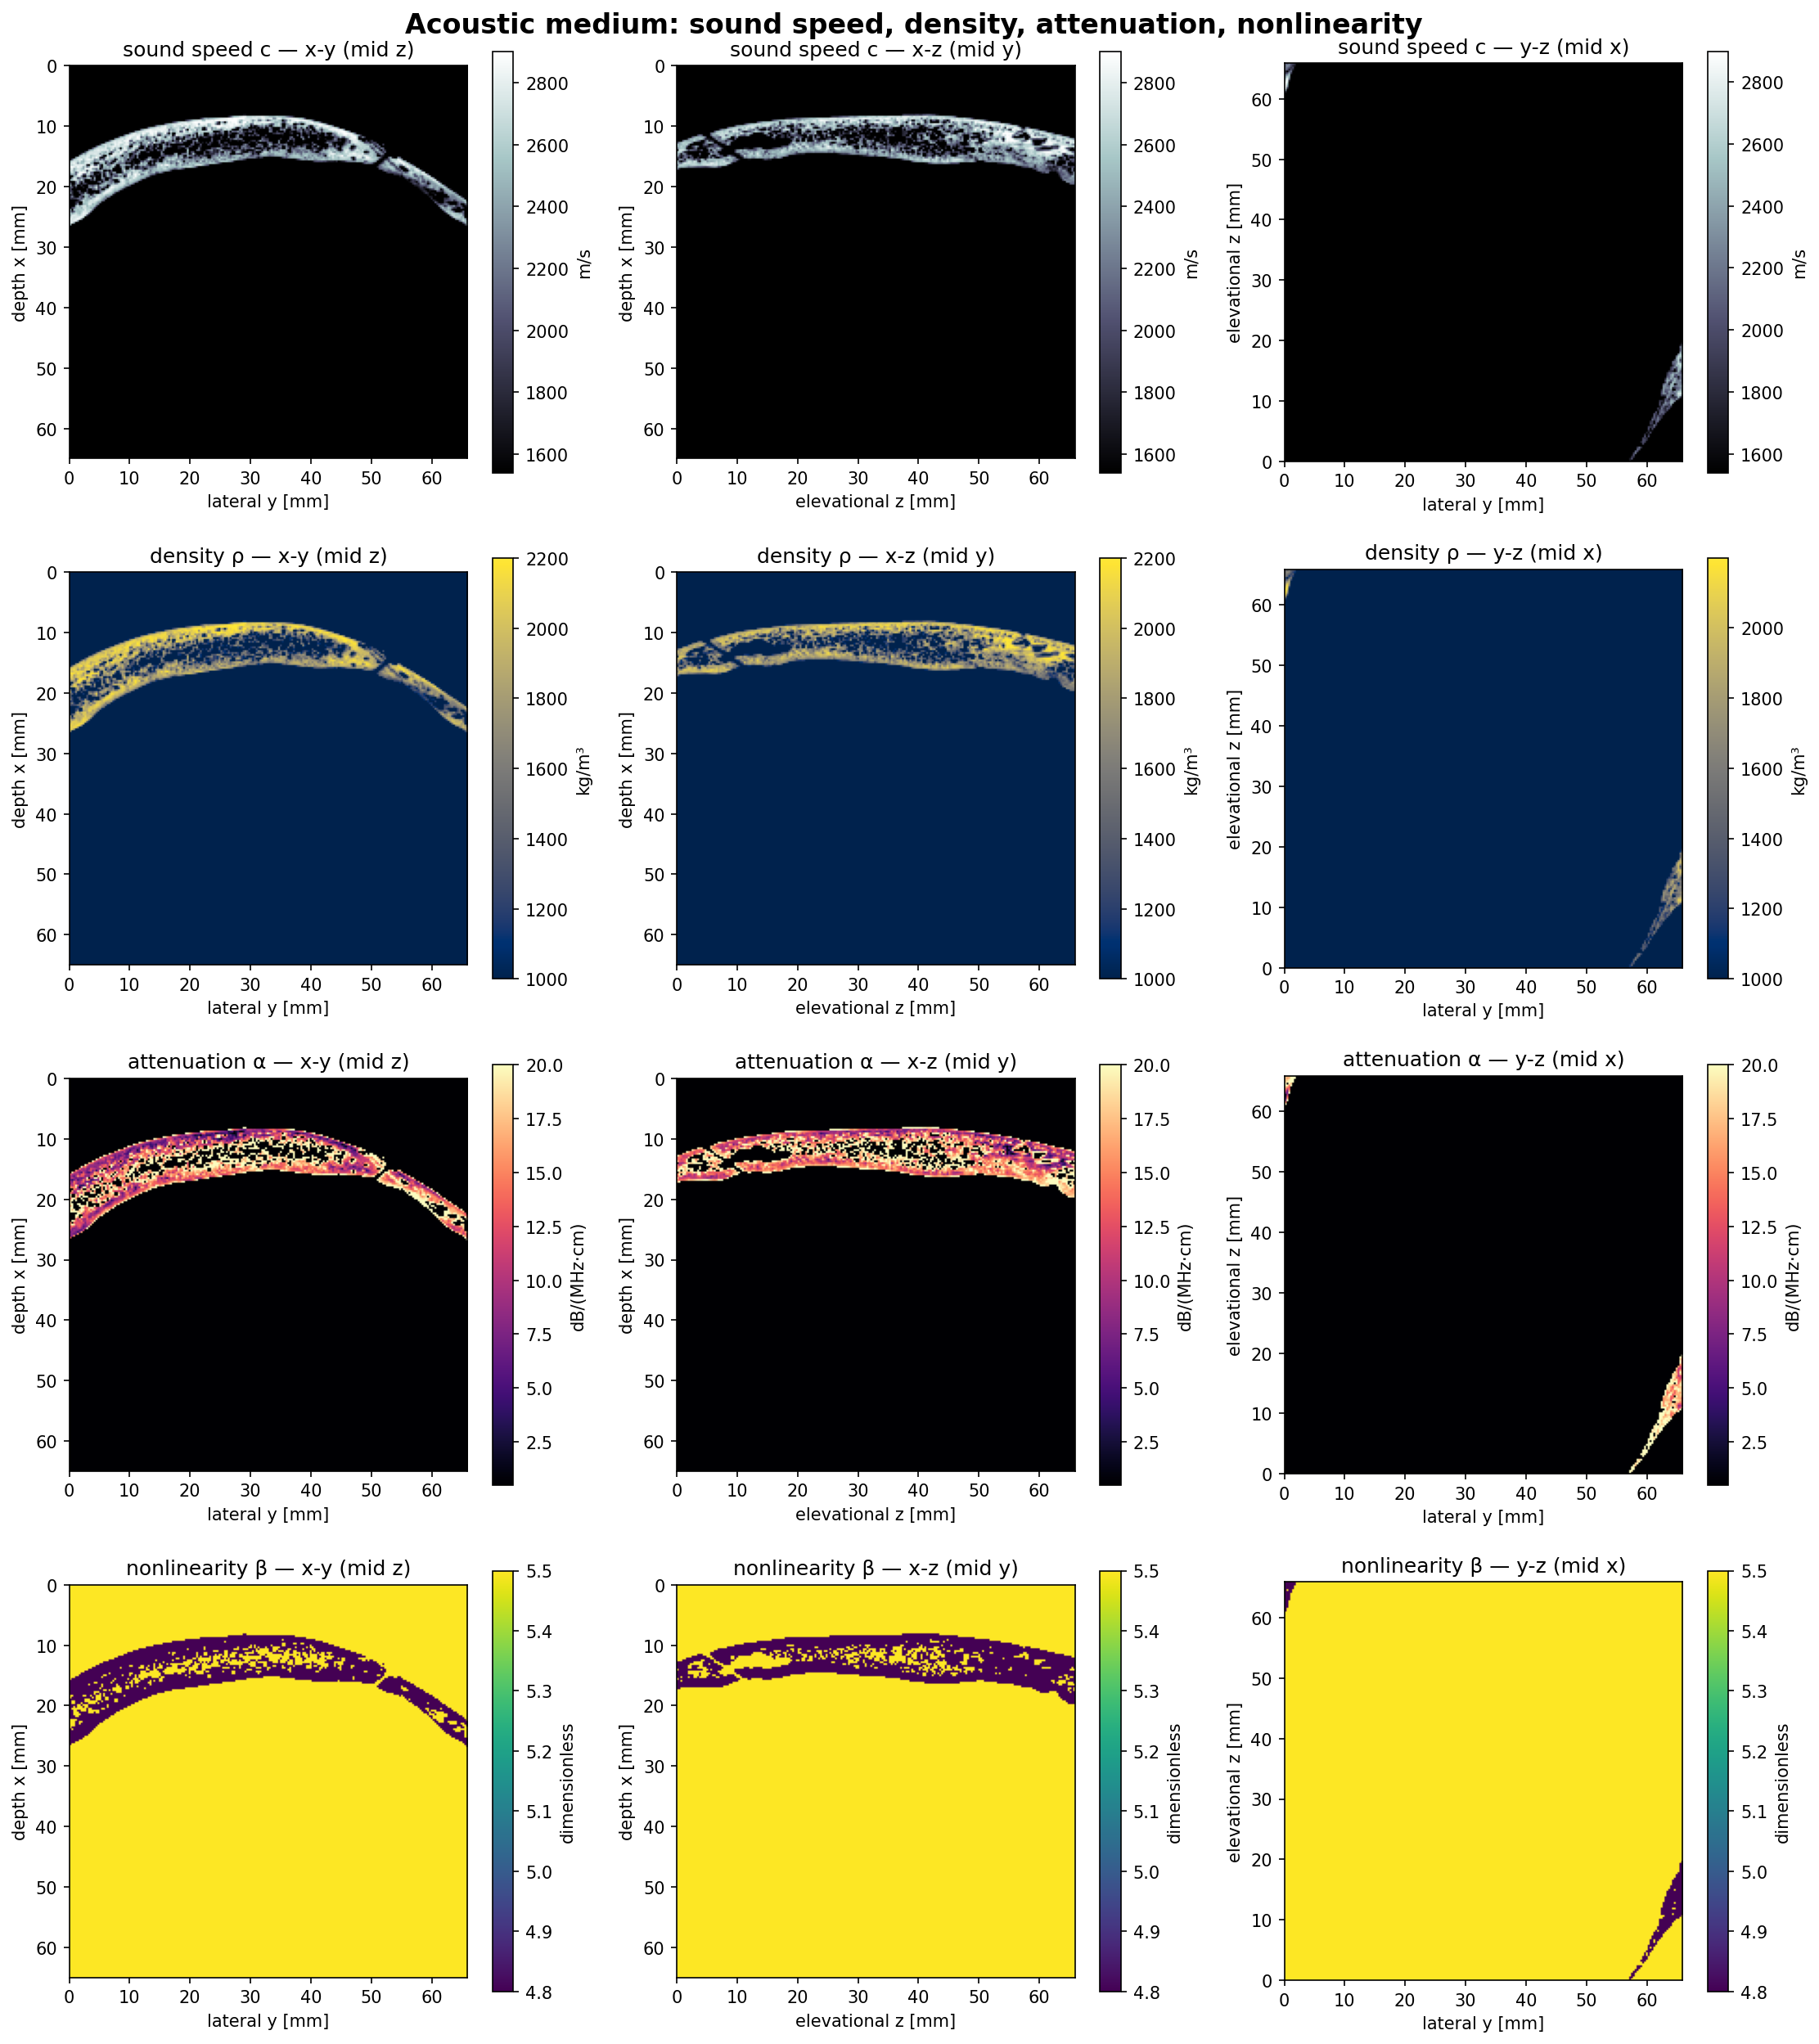
\includegraphics[width=\linewidth]{fig_inputs_medium.png}
\caption{Acoustic medium maps: sound speed $c$, density $\rho$, power-law attenuation $\alpha$, and nonlinearity coefficient $\beta$. Each row shows orthogonal mid-slices in x-y, x-z, and y-z.}\label{fig:medium}
\end{figure}

\subsection{Excitation waveform (per-pulse)}\label{sec:excitation}
\begin{figure}[h!]\centering
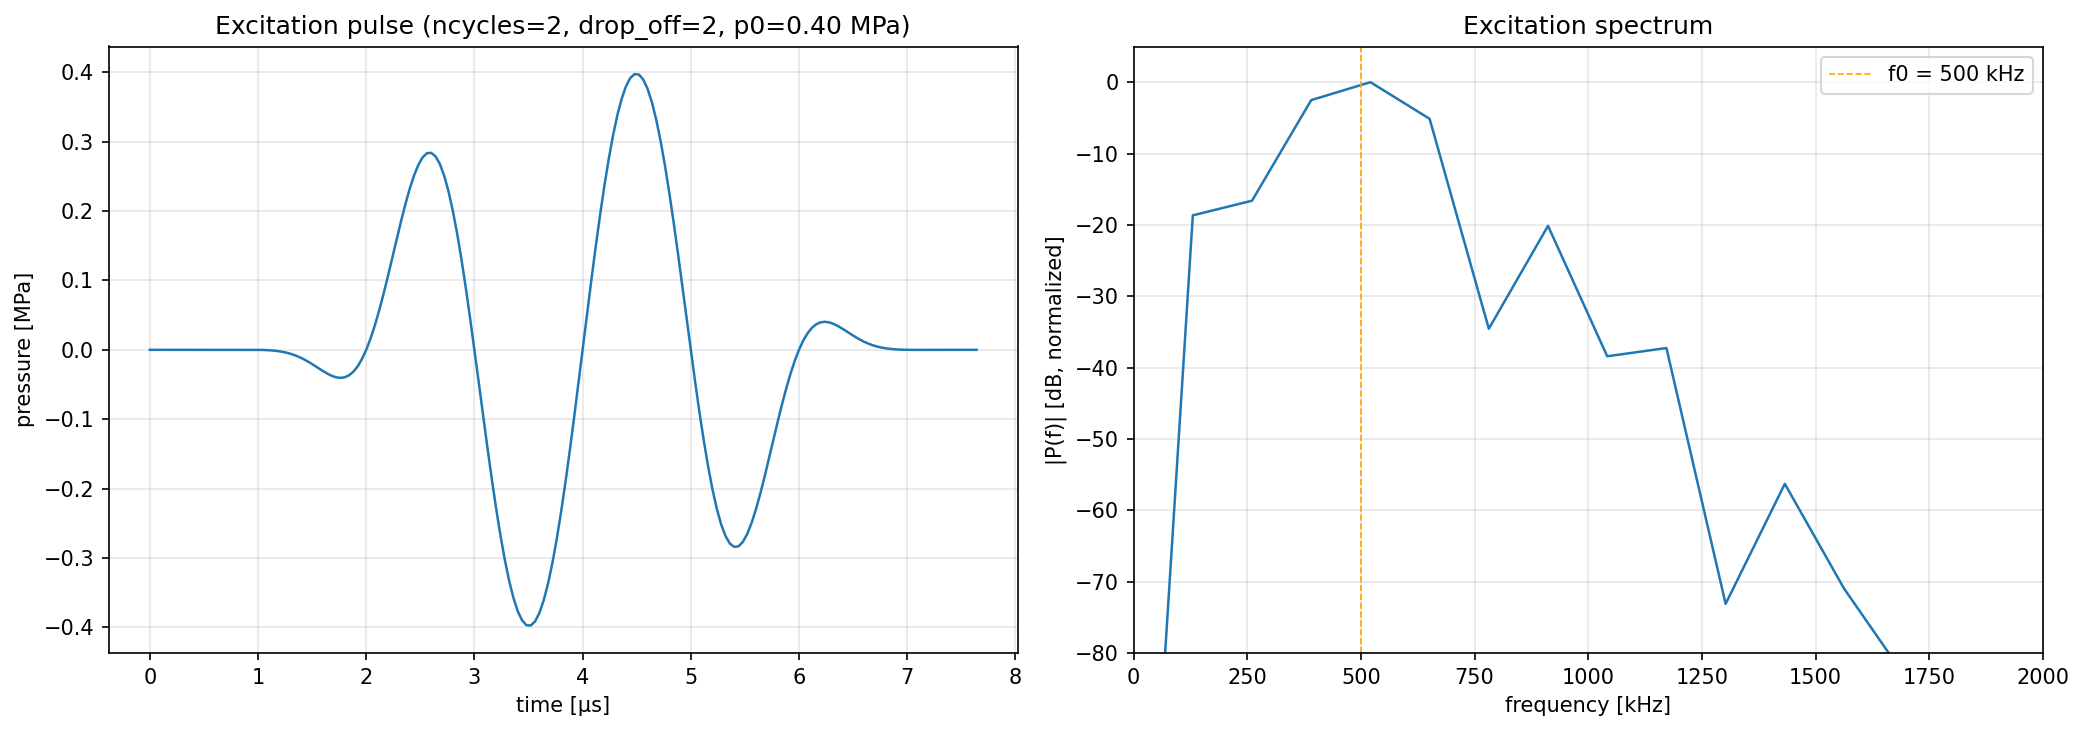
\includegraphics[width=\linewidth]{fig_inputs_excitation.png}
\caption{Per-voxel excitation pulse driving every bowl voxel (left) and its magnitude spectrum (right). All voxels fire the same pulse; geometric focusing arises from the bowl curvature.}\label{fig:excitation}
\end{figure}

\begin{table}[h!]
\centering
\scriptsize
\setlength{\tabcolsep}{6pt}
\begin{tabular}{lr|lr|lr}
\toprule
Cycles                  & 2 & Drop-off               & 2.0 & $p_0$                  & 0.40 MPa \\
$n_{\text{tic}}$        & 192   & Pulse duration         & 7.68 $\mu$s & CW correction          & 2.610 \\
Firing voxels           & 73638 & & & & \\
\bottomrule
\end{tabular}
\caption{Per-pulse excitation parameters derived from the source spec.}
\end{table}



\subsection{Neuromodulation sequence}\label{sec:sequence}

The FDTD captures the 80.0 ms
acoustic-radiation-force push window. The full session-level pulse schedule
that this push is embedded in is summarised below.


\begin{figure}[h!]\centering
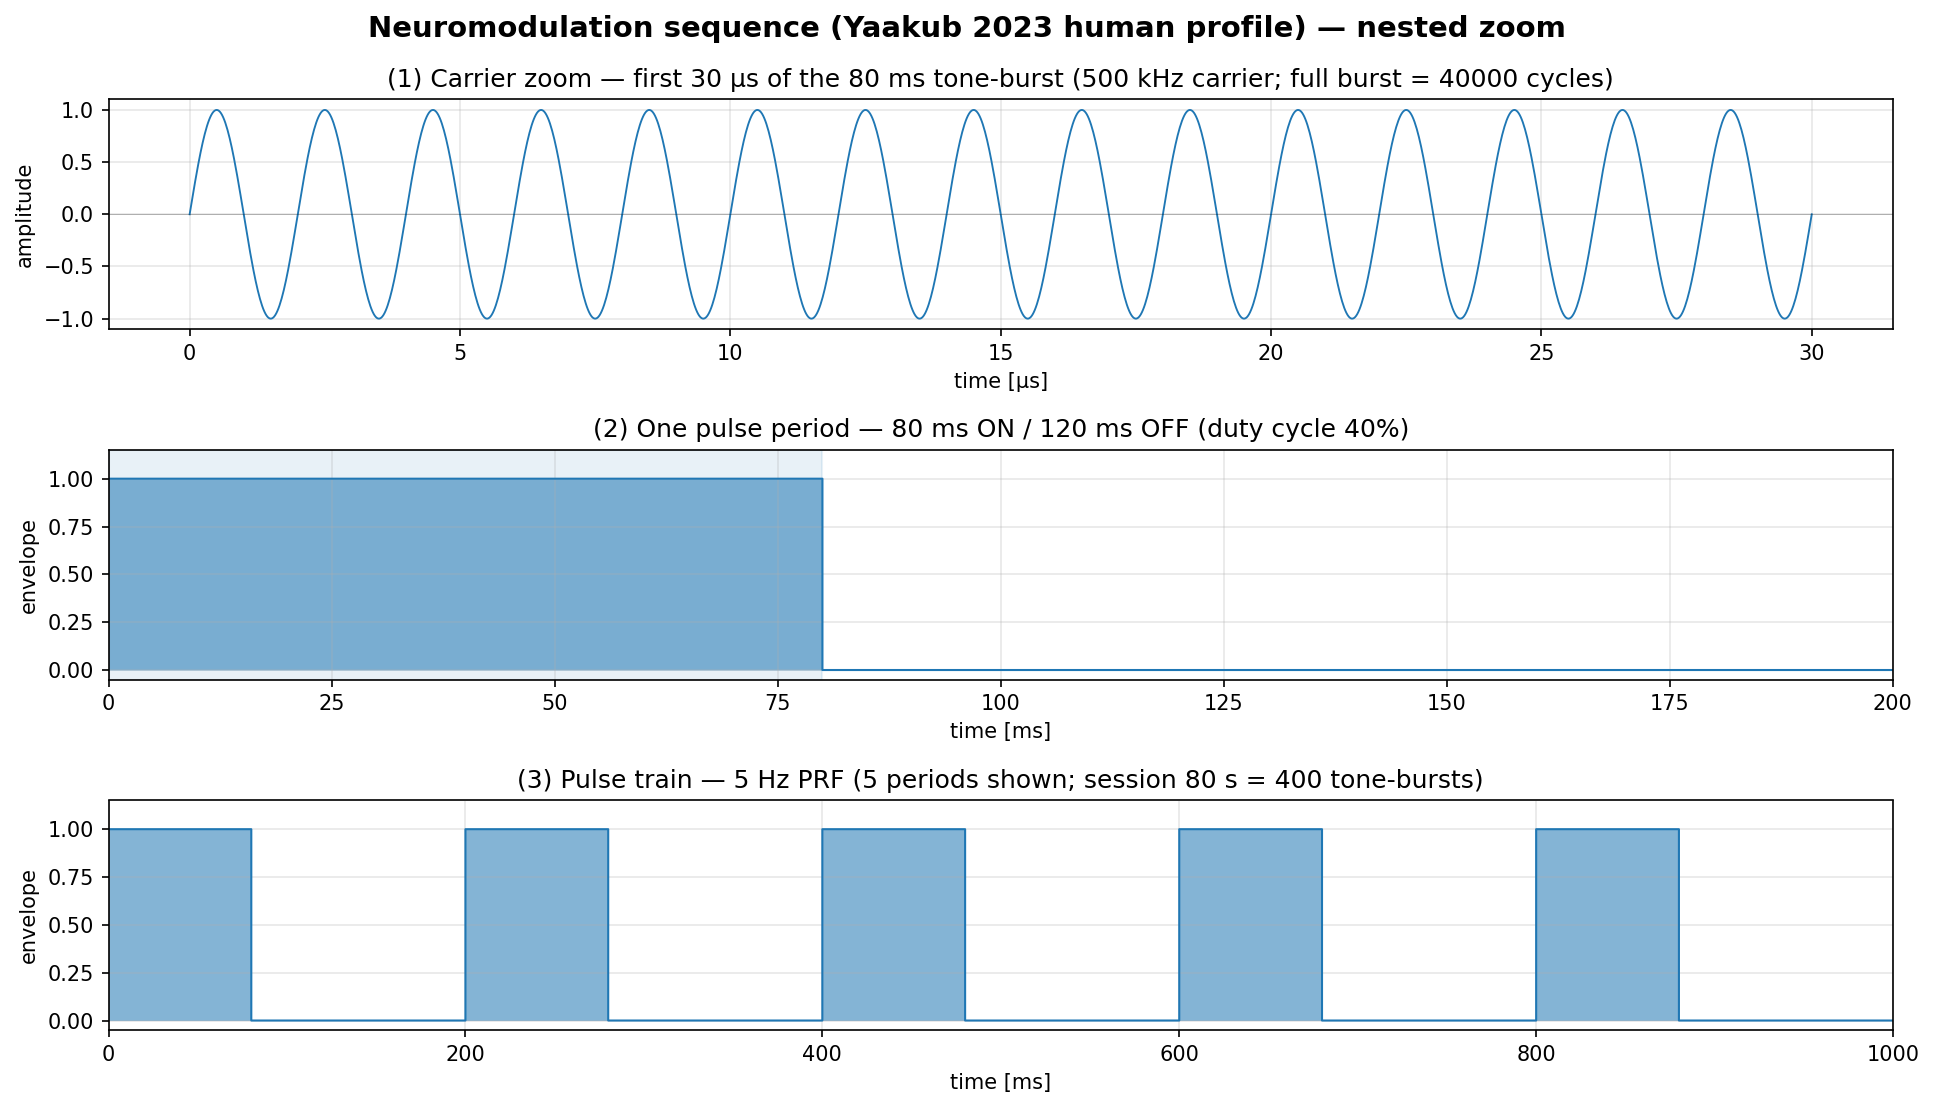
\includegraphics[width=\linewidth]{fig_inputs_sequence.png}
\caption{Yaakub 2023 human TUS protocol shown at three nested time scales: a zoom of the 500 kHz carrier within the tone-burst (top), one 200 ms pulse period showing 80 ms ON / 120 ms OFF (middle), and a 5 Hz pulse train across five periods (bottom).}\label{fig:sequence}
\end{figure}


\begin{table}[h!]
\centering
\scriptsize
\setlength{\tabcolsep}{6pt}
\begin{tabular}{lr|lr}
\toprule
Profile                         & yaakub\_human & Envelope                & rectangular CW tone-burst (no nested sub-bursts) \\
Carrier $f_0$                   & 500 kHz & Tone-burst duration     & 80 ms \\
PRF                             & 5.0 Hz & Pulse period            & 200 ms \\
Duty cycle                      & 40 \% & ISI (off-time)          & 120 ms \\
Session duration                & 80 s & Pulses per session      & 400 \\
ARF push window (FDTD)          & 80.0 ms & Target $I_{\text{SPPA}}$ & 30 W/cm\(^2\) \\
\bottomrule
\end{tabular}
\caption{Session-level TUS protocol (Yaakub 2023 human profile). The FDTD solves one tone-burst's ARF window; the table shows how that push is repeated in vivo.}
\end{table}




\section{Acoustic Outputs}\label{sec:acoustic_outputs}


\subsection{Pulse normalization and gating}\label{sec:pulse_norm}

The saved propagation map records a tone burst that is silent for most
of the saved window.  Recovering a continuous-wave-equivalent intensity
field requires two multiplicative corrections applied to the time-mean
of $p^2$: the silence correction lifts the full-window mean to the
active-pulse-window mean, and the cw correction (Gaussian-envelope
peak vs.\ sinusoidal RMS) lifts further to a continuous-wave reference.

\begin{table}[h!]
\centering
\scriptsize
\setlength{\tabcolsep}{6pt}
\begin{tabular}{lr|lr}
\toprule
$n_t$ saved (snapshots)            & 302                          & $n_{\mathrm{tic}}$ (source steps, full grid) & 192 \\
Sampling modulus time $\mathrm{smt}$ & 7          & Source steps saved $n_{\mathrm{tic}}/\mathrm{smt}$ & 27 \\
Silence correction $n_t / n_{\mathrm{src}}$ & 11.19 & CW correction (burst envelope) & 2.610 \\
\multicolumn{3}{r}{Pulse normalization (silence $\times$ cw)} & 29.20 \\
\bottomrule
\end{tabular}
\caption{Pulse-gating constants used to convert the saved $\langle p^2 \rangle$ field into a continuous-wave-equivalent intensity. The silence correction is the ratio of total saved snapshots to the number of active source steps (= $n_{\mathrm{tic}} / \mathrm{smt}$); the cw correction lifts the Gaussian-burst peak to a sinusoidal-RMS reference; their product is multiplied into $\langle p^2 \rangle$ before computing the intensity field rendered in Figs.~\ref{fig:acoustic_intensity}.}
\label{tab:pulse_norm}
\end{table}

\paragraph{Scaling the short-pulse output to a long-pulse exposure.}
The Fullwave run simulates a short Gaussian-windowed tone-burst of $n_{\mathrm{src}}$ active source steps embedded in $n_t$ saved snapshots, after which the source is silent and the field rings down.  The saved $\langle p^2 \rangle_{xyz}(t)$ has two regimes: an \emph{active-pulse window} where the spatial mean tracks the Gaussian burst envelope, and a \emph{silent ring-down} window where stored energy decays through the absorbing boundaries.  The two pulse-normalization constants in Table~\ref{tab:pulse_norm} convert this short-pulse output into the continuous-wave-equivalent intensity that an arbitrarily long real-world pulse would produce.

The \emph{silence correction} $n_t / n_{\mathrm{src}}$ is the duty-factor inverse: averaging $\langle p^2 \rangle$ over the full $n_t$-step window dilutes its value by the fraction of the window for which the source is actually emitting, so multiplying by $n_t / n_{\mathrm{src}}$ recovers the time-averaged $\langle p^2 \rangle$ of a CW source.  The \emph{cw correction} (typically $\approx 0.5$ for a half-sinusoid burst envelope, with the exact value tabulated) is the ratio of the burst's mean-square to a unit-amplitude CW sinusoid's mean-square; dividing $\langle p^2 \rangle$ by it lifts the Gaussian-burst peak to a sinusoidal-RMS reference.  Their product (silence $\times$ cw, also tabulated as ``Pulse normalization'') is the single multiplicative factor applied to the saved $\langle p^2 \rangle$ before the intensity field shown in Figs.~\ref{fig:acoustic_intensity} is computed.

Energy conservation then gives the relationship between the short and long pulses directly: a CW source delivering the same per-cycle PNP as the simulated burst deposits energy at a rate $n_t / n_{\mathrm{src}}$ times higher (the silence factor has the dimensions of a duty inverse), so total energy and time-averaged intensity scale by the same constant.  Peak quantities (PNP, PPP, MI) are unaffected by the correction; cumulative quantities ($I_{\mathrm{SPTA}}$, thermal index, $\Delta T$) all scale linearly with the pulse-normalization factor and therefore with simulated burst length once the geometry of the field has converged.

\subsection{Exposure metrics}\label{sec:exposure_metrics}

The metrics below are computed directly from the saved Fullwave acoustic
output (per-voxel pressure-time history, particle velocity, and
radiation-force density) on the downsampled validation grid, after the
pulse-normalization correction in Table~\ref{tab:pulse_norm}.  The
$\Delta T$ and strain-derived rows are produced by the bioheat and
shear-wave sub-pipelines and are reported in their own sections.

\begin{table}[h!]
\centering
\scriptsize
\setlength{\tabcolsep}{6pt}
\renewcommand{\arraystretch}{1.05}


\begin{tabular}{l r  l}
\toprule
\textbf{Quantity} & \textbf{Transcranial}  & \textbf{Unit} \\
\midrule
PNP                                  & 1.379        & MPa \\
PPP                                  & 1.517        & MPa \\
Mechanical Index                     & 1.95             & - \\
Thermal Index (soft tissue)          & 1.506        & - \\
Thermal Index (cranial)              & 7.905     & - \\
$I_{\mathrm{SPPA}}$                  & 73.68    & W/cm$^2$ \\
$I_{\mathrm{SPTA}}$                  & 26.526    & W/cm$^2$ \\
ARF density                          & 5470.53   & N/m$^3$ \\
$-6$\,dB volume                      & 174 & mm$^3$ \\
FWHM lateral ($y$)                   & 1.23      & mm \\
FWHM elevation ($z$)                 & 1.23      & mm \\
FWHM axial ($x$)                     & 1.23      & mm \\
$\langle I \rangle$ in $-6$\,dB vol  & 43.02   & W/cm$^2$ \\
Peak particle velocity               & 1.018e-04 & m/s \\
ARF impulse / pulse                  & 1.969e+00 & Pa$\cdot$s \\
\bottomrule
\end{tabular}
\caption{Acoustic exposure metrics from the FDTD output.  ISPTA uses the within-burst duty cycle of 0.36; pulse duration 360.00 $\mu$s.  Strain-derived and bioheat-derived rows ($\Delta T$, peak strain, peak strain rate, peak strain gradient) are reported in subsequent sections.}
\label{tab:acoustic_outputs}
\end{table}

\subsection{Pressure snapshots — early / focal / post-focal}\label{sec:pressure_snapshots}
\begin{figure}[h!]\centering
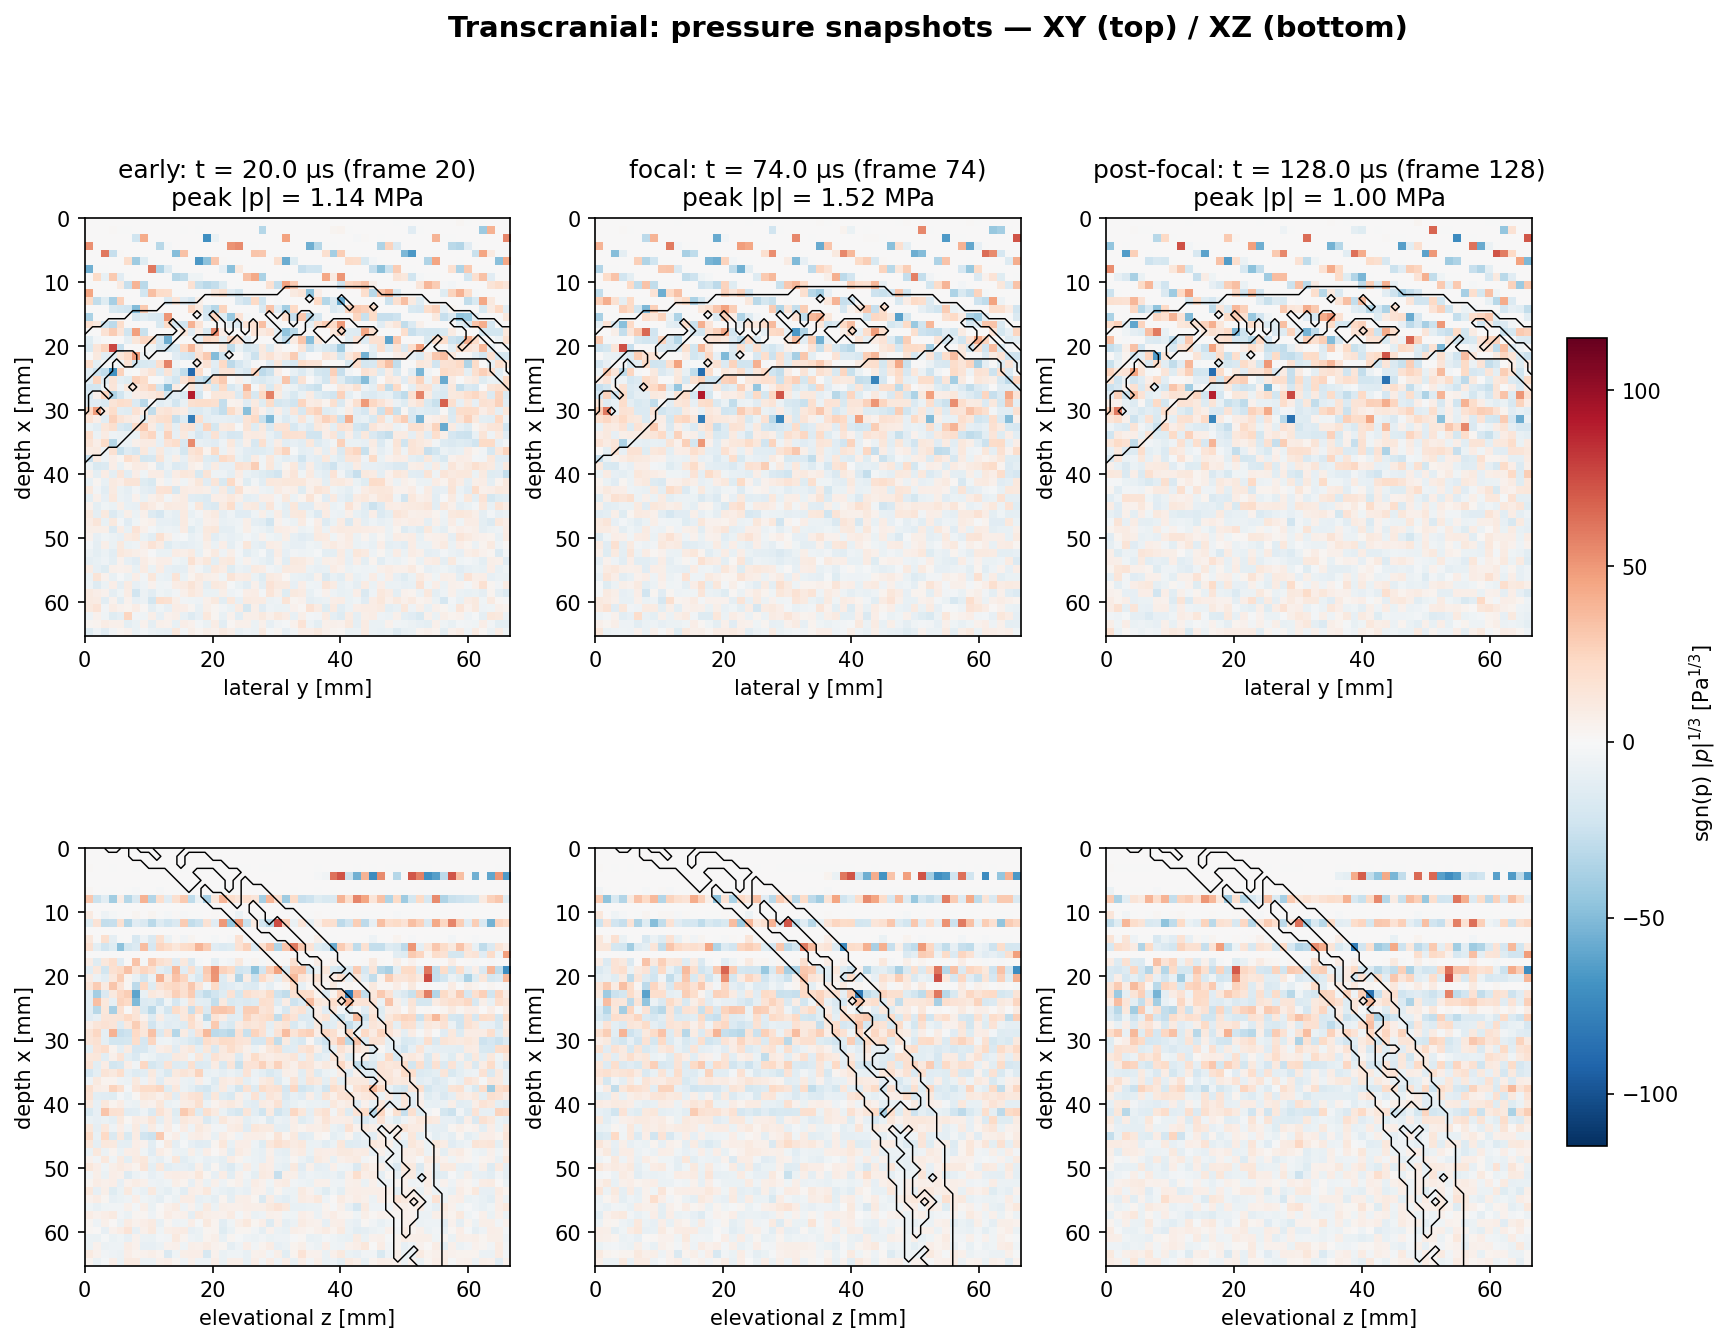
\includegraphics[width=\linewidth]{acoustic_pressure_snapshots.png}
\caption{Acoustic pressure snapshots at three timepoints: early (wave entering the domain), focal (global peak $|p|$), and post-focal (wave past the geometric focus). Top row: XY mid-z slices; bottom row: XZ mid-y slices. Colorscale is the sign-preserving cube-root compression $\mathrm{sgn}(p)\,|p|^{1/3}$ to make low-amplitude propagating wavefronts visible alongside the focal peak. Black contour outlines the skull mask ($c > 1600$\,m/s). Frame indices, timepoints, and per-frame peak $|p|$ in MPa are annotated above each panel.\\
{\scriptsize Frames: early $t=20.0$ µs (peak $|p|=1.14$ MPa) | focal $t=74.0$ µs (peak $|p|=1.52$ MPa) | post $t=128.0$ µs (peak $|p|=1.00$ MPa). Global peak $|p|=1.52$ MPa.}}\label{fig:pressure_snapshots}
\end{figure}

\subsection{Focal intensity — slices and 3D iso-surfaces}\label{sec:intensity}
\begin{figure}[h!]\centering
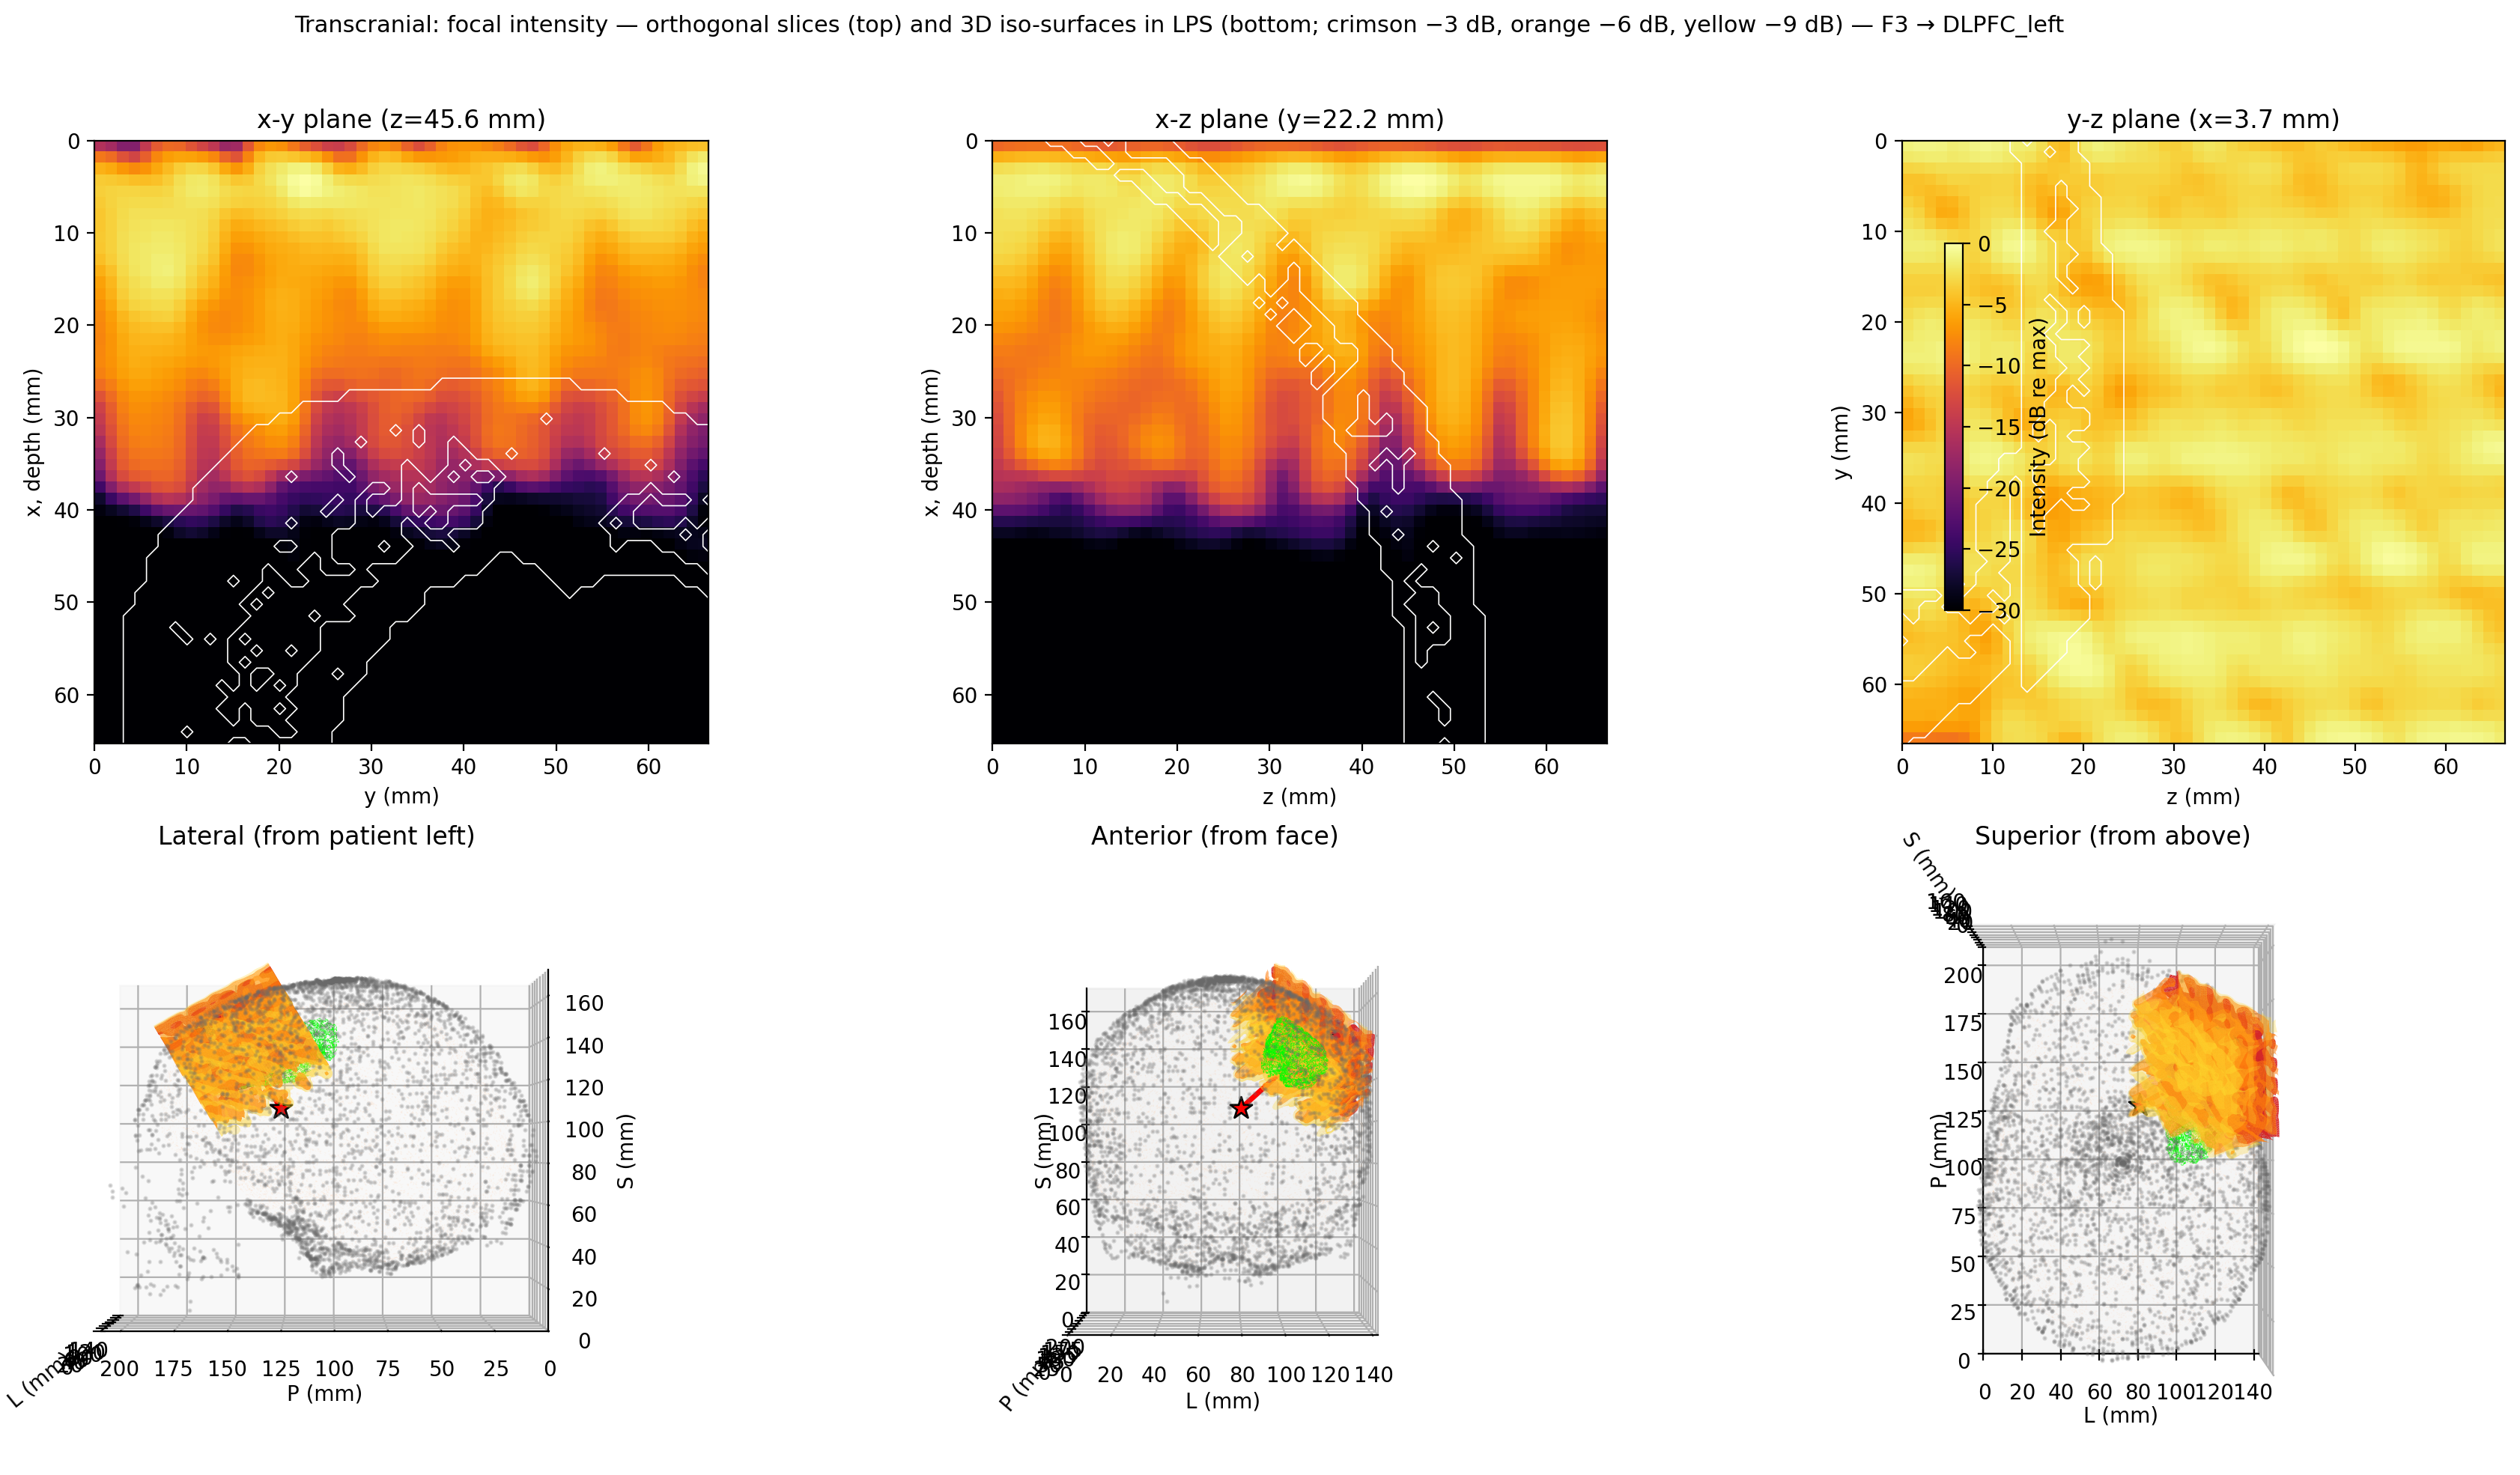
\includegraphics[width=\linewidth]{acoustic_intensity_combined.png}
\caption{Top: orthogonal slices of intensity through the focal voxel in dB re max, with the skull mask ($c > 1700$\,m/s) contoured in white. Bottom: same focal lobe rendered in LPS coordinates with the skull point cloud, pial brain mesh, target ROI (lime), and bowl wireframe (steelblue), viewed from three camera angles. Nested iso-surfaces: crimson $-3$ dB, orange $-6$ dB, yellow $-9$ dB.}\label{fig:acoustic_intensity}
\end{figure}











\section{Reproducibility}\label{sec:repro}
\begin{table}[h!]
\centering
\scriptsize
\setlength{\tabcolsep}{6pt}
\begin{tabular}{lr|lr}
\toprule
Host                & \texttt{germignaga} & Python              & \texttt{3.10.12} \\
Fullwave path       & \texttt{\textasciitilde{}/fullwave25-speckle/fullwave} & Fullwave SHA        & \texttt{2f8dea3} \\
Neuromod SHA        & \texttt{65ab845} & Acoustoelastic SHA  & \texttt{n/a} \\
Generated at        & 2026-05-01T18:07:01-04:00 & & \\
\bottomrule
\end{tabular}
\caption{Build manifest captured at report generation.}
\end{table}

\end{document}
